
%%%%%%%%%%%%%%%%%%%%%%% file typeinst.tex %%%%%%%%%%%%%%%%%%%%%%%%%
%
% This is the LaTeX source for the instructions to authors using
% the LaTeX document class 'llncs.cls' for contributions to
% the Lecture Notes in Computer Sciences series.
% http://www.springer.com/lncs       Springer Heidelberg 2006/05/04
%
% It may be used as a template for your own input - copy it
% to a new file with a new name and use it as the basis
% for your article.
%
% NB: the document class 'llncs' has its own and detailed documentation, see
% ftp://ftp.springer.de/data/pubftp/pub/tex/latex/llncs/latex2e/llncsdoc.pdf
%
%%%%%%%%%%%%%%%%%%%%%%%%%%%%%%%%%%%%%%%%%%%%%%%%%%%%%%%%%%%%%%%%%%%


\documentclass[runningheads,a4paper]{llncs}

\usepackage{amssymb}
\setcounter{tocdepth}{3}
\usepackage{graphicx}

\usepackage{url}
\urldef{\mailsa}\path|{alfred.hofmann, ursula.barth, ingrid.haas, frank.holzwarth,|
\urldef{\mailsb}\path|anna.kramer, leonie.kunz, christine.reiss, nicole.sator,|
\urldef{\mailsc}\path|erika.siebert-cole, peter.strasser, lncs}@springer.com|    
\newcommand{\keywords}[1]{\par\addvspace\baselineskip
\noindent\keywordname\enspace\ignorespaces#1}

\begin{document}

\mainmatter  % start of an individual contribution

% first the title is needed
\title{Lecture Notes in Computer Science:\\Authors' Instructions
for the Preparation\\of Camera-Ready
Contributions\\to LNCS/LNAI/LNBI Proceedings}

% a short form should be given in case it is too long for the running head
\titlerunning{Lecture Notes in Computer Science: Authors' Instructions}

% the name(s) of the author(s) follow(s) next
%
% NB: Chinese authors should write their first names(s) in front of
% their surnames. This ensures that the names appear correctly in
% the running heads and the author index.
%
\author{Alfred Hofmann%
\thanks{Please note that the LNCS Editorial assumes that all authors have used
the western naming convention, with given names preceding surnames. This determines
the structure of the names in the running heads and the author index.}%
\and Ursula Barth\and Ingrid Haas\and Frank Holzwarth\and\\
Anna Kramer\and Leonie Kunz\and Christine Rei\ss\and\\
Nicole Sator\and Erika Siebert-Cole\and Peter Stra\ss er}
%
\authorrunning{Lecture Notes in Computer Science: Authors' Instructions}
% (feature abused for this document to repeat the title also on left hand pages)

% the affiliations are given next; don't give your e-mail address
% unless you accept that it will be published
\institute{Springer-Verlag, Computer Science Editorial,\\
Tiergartenstr. 17, 69121 Heidelberg, Germany\\
\mailsa\\
\mailsb\\
\mailsc\\
\url{http://www.springer.com/lncs}}

%
% NB: a more complex sample for affiliations and the mapping to the
% corresponding authors can be found in the file "llncs.dem"
% (search for the string "\mainmatter" where a contribution starts).
% "llncs.dem" accompanies the document class "llncs.cls".
%

\toctitle{Lecture Notes in Computer Science}
\tocauthor{Authors' Instructions}
\maketitle


\begin{abstract}
The abstract should summarize the contents of the paper and should
contain at least 70 and at most 150 words. It should be written using the
\emph{abstract} environment.
\keywords{We would like to encourage you to list your keywords within
the abstract section}
\end{abstract}


\section{Introduction}

You are strongly encouraged to use \LaTeXe{} for the
preparation of your camera-ready manuscript together with the
corresponding Springer class file \verb+llncs.cls+. Only if you use
\LaTeXe{} can hyperlinks be generated in the online version
of your manuscript.

The \LaTeX{} source of this instruction file for \LaTeX{} users may be
used as a template. This is
located in the ``authors'' subdirectory in
\url{ftp://ftp.springer.de/pub/tex/latex/llncs/latex2e/instruct/} and
entitled \texttt{typeinst.tex}. There is a separate package for Word 
users. Kindly send the final and checked source
and PDF files of your paper to the Contact Volume Editor. This is
usually one of the organizers of the conference. You should make sure
that the \LaTeX{} and the PDF files are identical and correct and that
only one version of your paper is sent. It is not possible to update
files at a later stage. Please note that we do not need the printed
paper.

We would like to draw your attention to the fact that it is not possible
to modify a paper in any way, once it has been published. This applies
to both the printed book and the online version of the publication.
Every detail, including the order of the names of the authors, should
be checked before the paper is sent to the Volume Editors.

\subsection{Checking the PDF File}

Kindly assure that the Contact Volume Editor is given the name and email
address of the contact author for your paper. The Contact Volume Editor
uses these details to compile a list for our production department at
SPS in India. Once the files have been worked upon, SPS sends a copy of
the final pdf of each paper to its contact author. The contact author is
asked to check through the final pdf to make sure that no errors have
crept in during the transfer or preparation of the files. This should
not be seen as an opportunity to update or copyedit the papers, which is
not possible due to time constraints. Only errors introduced during the
preparation of the files will be corrected.

This round of checking takes place about two weeks after the files have
been sent to the Editorial by the Contact Volume Editor, i.e., roughly
seven weeks before the start of the conference for conference
proceedings, or seven weeks before the volume leaves the printer's, for
post-proceedings. If SPS does not receive a reply from a particular
contact author, within the timeframe given, then it is presumed that the
author has found no errors in the paper. The tight publication schedule
of LNCS does not allow SPS to send reminders or search for alternative
email addresses on the Internet.

In some cases, it is the Contact Volume Editor that checks all the final
pdfs. In such cases, the authors are not involved in the checking phase.

\subsection{Additional Information Required by the Volume Editor}

If you have more than one surname, please make sure that the Volume Editor
knows how you are to be listed in the author index.

\subsection{Copyright Forms}

The copyright form may be downloaded from the ``For Authors"
(Information for LNCS Authors) section of the LNCS Website:
\texttt{www.springer.com/lncs}. Please send your signed copyright form
to the Contact Volume Editor, either as a scanned pdf or by fax or by
courier. One author may sign on behalf of all of the other authors of a
particular paper. Digital signatures are acceptable.

\section{Paper Preparation}

Springer provides you with a complete integrated \LaTeX{} document class
(\texttt{llncs.cls}) for multi-author books such as those in the LNCS
series. Papers not complying with the LNCS style will be reformatted.
This can lead to an increase in the overall number of pages. We would
therefore urge you not to squash your paper.

Please always cancel any superfluous definitions that are
not actually used in your text. If you do not, these may conflict with
the definitions of the macro package, causing changes in the structure
of the text and leading to numerous mistakes in the proofs.

If you wonder what \LaTeX{} is and where it can be obtained, see the
``\textit{LaTeX project site}'' (\url{http://www.latex-project.org})
and especially the webpage ``\textit{How to get it}''
(\url{http://www.latex-project.org/ftp.html}) respectively.

When you use \LaTeX\ together with our document class file,
\texttt{llncs.cls},
your text is typeset automatically in Computer Modern Roman (CM) fonts.
Please do
\emph{not} change the preset fonts. If you have to use fonts other
than the preset fonts, kindly submit these with your files.

Please use the commands \verb+\label+ and \verb+\ref+ for
cross-references and the commands \verb+\bibitem+ and \verb+\cite+ for
references to the bibliography, to enable us to create hyperlinks at
these places.

For preparing your figures electronically and integrating them into
your source file we recommend using the standard \LaTeX{} \verb+graphics+ or
\verb+graphicx+ package. These provide the \verb+\includegraphics+ command.
In general, please refrain from using the \verb+\special+ command.

Remember to submit any further style files and
fonts you have used together with your source files.

\subsubsection{Headings.}

Headings should be capitalized
(i.e., nouns, verbs, and all other words
except articles, prepositions, and conjunctions should be set with an
initial capital) and should,
with the exception of the title, be aligned to the left.
Words joined by a hyphen are subject to a special rule. If the first
word can stand alone, the second word should be capitalized.

Here are some examples of headings: ``Criteria to Disprove
Context-Freeness of Collage Language", ``On Correcting the Intrusion of
Tracing Non-deterministic Programs by Software", ``A User-Friendly and
Extendable Data Distribution System", ``Multi-flip Networks:
Parallelizing GenSAT", ``Self-determinations of Man".

\subsubsection{Lemmas, Propositions, and Theorems.}

The numbers accorded to lemmas, propositions, and theorems, etc. should
appear in consecutive order, starting with Lemma 1, and not, for
example, with Lemma 11.

\subsection{Figures}

For \LaTeX\ users, we recommend using the \emph{graphics} or \emph{graphicx}
package and the \verb+\includegraphics+ command.

Please check that the lines in line drawings are not
interrupted and are of a constant width. Grids and details within the
figures must be clearly legible and may not be written one on top of
the other. Line drawings should have a resolution of at least 800 dpi
(preferably 1200 dpi). The lettering in figures should have a height of
2~mm (10-point type). Figures should be numbered and should have a
caption which should always be positioned \emph{under} the figures, in
contrast to the caption belonging to a table, which should always appear
\emph{above} the table; this is simply achieved as matter of sequence in
your source.

Please center the figures or your tabular material by using the \verb+\centering+
declaration. Short captions are centered by default between the margins
and typeset in 9-point type (Fig.~\ref{fig:example} shows an example).
The distance between text and figure is preset to be about 8~mm, the
distance between figure and caption about 6~mm.

To ensure that the reproduction of your illustrations is of a reasonable
quality, we advise against the use of shading. The contrast should be as
pronounced as possible.

If screenshots are necessary, please make sure that you are happy with
the print quality before you send the files.
\begin{figure}
\centering
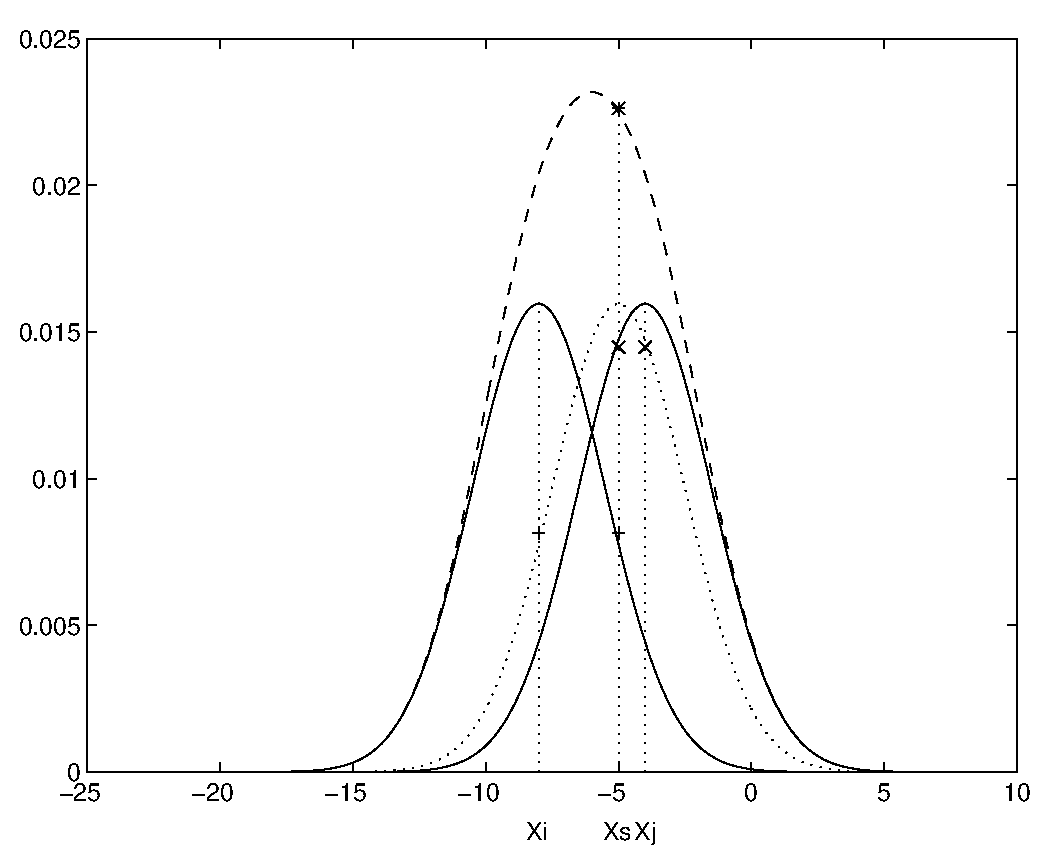
\includegraphics[height=6.2cm]{eijkel2}
\caption{One kernel at $x_s$ (\emph{dotted kernel}) or two kernels at
$x_i$ and $x_j$ (\textit{left and right}) lead to the same summed estimate
at $x_s$. This shows a figure consisting of different types of
lines. Elements of the figure described in the caption should be set in
italics, in parentheses, as shown in this sample caption.}
\label{fig:example}
\end{figure}

Please define figures (and tables) as floating objects. Please avoid
using optional location parameters like ``\verb+[h]+" for ``here".

\paragraph{Remark 1.}

In the printed volumes, illustrations are generally black and white
(halftones), and only in exceptional cases, and if the author is
prepared to cover the extra cost for color reproduction, are colored
pictures accepted. Colored pictures are welcome in the electronic
version free of charge. If you send colored figures that are to be
printed in black and white, please make sure that they really are
legible in black and white. Some colors as well as the contrast of
converted colors show up very poorly when printed in black and white.

\subsection{Formulas}

Displayed equations or formulas are centered and set on a separate
line (with an extra line or halfline space above and below). Displayed
expressions should be numbered for reference. The numbers should be
consecutive within each section or within the contribution,
with numbers enclosed in parentheses and set on the right margin --
which is the default if you use the \emph{equation} environment, e.g.,
\begin{equation}
  \psi (u) = \int_{o}^{T} \left[\frac{1}{2}
  \left(\Lambda_{o}^{-1} u,u\right) + N^{\ast} (-u)\right] dt \;  .
\end{equation}

Equations should be punctuated in the same way as ordinary
text but with a small space before the end punctuation mark.

\subsection{Footnotes}

The superscript numeral used to refer to a footnote appears in the text
either directly after the word to be discussed or -- in relation to a
phrase or a sentence -- following the punctuation sign (comma,
semicolon, or period). Footnotes should appear at the bottom of
the
normal text area, with a line of about 2~cm set
immediately above them.\footnote{The footnote numeral is set flush left
and the text follows with the usual word spacing.}

\subsection{Program Code}

Program listings or program commands in the text are normally set in
typewriter font, e.g., CMTT10 or Courier.

\medskip

\noindent
{\it Example of a Computer Program}
\begin{verbatim}
program Inflation (Output)
  {Assuming annual inflation rates of 7%, 8%, and 10%,...
   years};
   const
     MaxYears = 10;
   var
     Year: 0..MaxYears;
     Factor1, Factor2, Factor3: Real;
   begin
     Year := 0;
     Factor1 := 1.0; Factor2 := 1.0; Factor3 := 1.0;
     WriteLn('Year  7% 8% 10%'); WriteLn;
     repeat
       Year := Year + 1;
       Factor1 := Factor1 * 1.07;
       Factor2 := Factor2 * 1.08;
       Factor3 := Factor3 * 1.10;
       WriteLn(Year:5,Factor1:7:3,Factor2:7:3,Factor3:7:3)
     until Year = MaxYears
end.
\end{verbatim}
%
\noindent
{\small (Example from Jensen K., Wirth N. (1991) Pascal user manual and
report. Springer, New York)}

\subsection{Citations}

For citations in the text please use
square brackets and consecutive numbers: \cite{jour}, \cite{lncschap},
\cite{proceeding1} -- provided automatically
by \LaTeX 's \verb|\cite| \dots\verb|\bibitem| mechanism.

\subsection{Page Numbering and Running Heads}

There is no need to include page numbers. If your paper title is too
long to serve as a running head, it will be shortened. Your suggestion
as to how to shorten it would be most welcome.

\section{LNCS Online}

The online version of the volume will be available in LNCS Online.
Members of institutes subscribing to the Lecture Notes in Computer
Science series have access to all the pdfs of all the online
publications. Non-subscribers can only read as far as the abstracts. If
they try to go beyond this point, they are automatically asked, whether
they would like to order the pdf, and are given instructions as to how
to do so.

Please note that, if your email address is given in your paper,
it will also be included in the meta data of the online version.

\section{BibTeX Entries}

The correct BibTeX entries for the Lecture Notes in Computer Science
volumes can be found at the following Website shortly after the
publication of the book:
\url{http://www.informatik.uni-trier.de/~ley/db/journals/lncs.html}

\subsubsection*{Acknowledgments.} The heading should be treated as a
subsubsection heading and should not be assigned a number.

\section{The References Section}\label{references}

In order to permit cross referencing within LNCS-Online, and eventually
between different publishers and their online databases, LNCS will,
from now on, be standardizing the format of the references. This new
feature will increase the visibility of publications and facilitate
academic research considerably. Please base your references on the
examples below. References that don't adhere to this style will be
reformatted by Springer. You should therefore check your references
thoroughly when you receive the final pdf of your paper.
The reference section must be complete. You may not omit references.
Instructions as to where to find a fuller version of the references are
not permissible.

We only accept references written using the latin alphabet. If the title
of the book you are referring to is in Russian or Chinese, then please write
(in Russian) or (in Chinese) at the end of the transcript or translation
of the title.

The following section shows a sample reference list with entries for
journal articles \cite{jour}, an LNCS chapter \cite{lncschap}, a book
\cite{book}, proceedings without editors \cite{proceeding1} and
\cite{proceeding2}, as well as a URL \cite{url}.
Please note that proceedings published in LNCS are not cited with their
full titles, but with their acronyms!

\begin{thebibliography}{4}

\bibitem{jour} Smith, T.F., Waterman, M.S.: Identification of Common Molecular
Subsequences. J. Mol. Biol. 147, 195--197 (1981)

\bibitem{lncschap} May, P., Ehrlich, H.C., Steinke, T.: ZIB Structure Prediction Pipeline:
Composing a Complex Biological Workflow through Web Services. In: Nagel,
W.E., Walter, W.V., Lehner, W. (eds.) Euro-Par 2006. LNCS, vol. 4128,
pp. 1148--1158. Springer, Heidelberg (2006)

\bibitem{book} Foster, I., Kesselman, C.: The Grid: Blueprint for a New Computing
Infrastructure. Morgan Kaufmann, San Francisco (1999)

\bibitem{proceeding1} Czajkowski, K., Fitzgerald, S., Foster, I., Kesselman, C.: Grid
Information Services for Distributed Resource Sharing. In: 10th IEEE
International Symposium on High Performance Distributed Computing, pp.
181--184. IEEE Press, New York (2001)

\bibitem{proceeding2} Foster, I., Kesselman, C., Nick, J., Tuecke, S.: The Physiology of the
Grid: an Open Grid Services Architecture for Distributed Systems
Integration. Technical report, Global Grid Forum (2002)

\bibitem{url} National Center for Biotechnology Information, \url{http://www.ncbi.nlm.nih.gov}

\end{thebibliography}


\section*{Appendix: Springer-Author Discount}

LNCS authors are entitled to a 33.3\% discount off all Springer
publications. Before placing an order, the author should send an email, 
giving full details of his or her Springer publication,
to \url{orders-HD-individuals@springer.com} to obtain a so-called token. This token is a
number, which must be entered when placing an order via the Internet, in
order to obtain the discount.

\section{Checklist of Items to be Sent to Volume Editors}
Here is a checklist of everything the volume editor requires from you:


\begin{itemize}
\settowidth{\leftmargin}{{\Large$\square$}}\advance\leftmargin\labelsep
\itemsep8pt\relax
\renewcommand\labelitemi{{\lower1.5pt\hbox{\Large$\square$}}}

\item The final \LaTeX{} source files
\item A final PDF file
\item A copyright form, signed by one author on behalf of all of the
authors of the paper.
\item A readme giving the name and email address of the
corresponding author.
\end{itemize}
\end{document}
